% -*- latex -*-
%%%%%%%%%%%%%%%%%%%%%%%%%%%%%%%%%%%%%%%%%%%%%%%%%%%%%%%%%%%%%%%%
%%%%%%%%%%%%%%%%%%%%%%%%%%%%%%%%%%%%%%%%%%%%%%%%%%%%%%%%%%%%%%%%
%%%%
%%%% This text file is part of the source of slides for
%%%% `Introduction to High-Performance Scientific Computing'
%%%% by Victor Eijkhout, copyright 2012
%%%%
%%%%%%%%%%%%%%%%%%%%%%%%%%%%%%%%%%%%%%%%%%%%%%%%%%%%%%%%%%%%%%%%
%%%%%%%%%%%%%%%%%%%%%%%%%%%%%%%%%%%%%%%%%%%%%%%%%%%%%%%%%%%%%%%%

\Level 1 {Multicore block algorithms}

\newcommand\chol{\mathop{\mathrm{Chol}}}

\begin{frame}{Cholesky algorithm}
\[ \chol
\begin{pmatrix}
  A_{11}&A_{21}^t\\ A_{21}&A_{22}
\end{pmatrix} = LL^t\qquad\hbox{where}\quad L=
\begin{pmatrix}
  L_{11}&0\\ \tilde A_{21} &\chol(A_{22}-\tilde A_{21}\tilde A_{21}^t)
\end{pmatrix}
\]
and where $\tilde A_{21}=A_{21}L_{11}\invt,$ $A_{11}=L_{11}L_{11}^t$.  
\end{frame}

\begin{frame}{Implementation}
  \begin{tabbing}
    for \=$k=1,\mathrm{nblocks}$:\\
    \>\n{Chol}: factor $L_kL_k^t\leftarrow A_{kk}$\\
    \>\n{Trsm}: solve $\tilde A_{>k,k} \leftarrow A_{>k,k}L_k\invt$\\
    \>\n{Gemm}: form the product $\tilde A_{>k,k}\tilde A_{>k,k}^t$\\
    \>\n{Syrk}: symmmetric rank-$k$ update
    $A_{>k,>k}\leftarrow A_{>k,>k}-\tilde A_{>k,k}\tilde A_{>k,k}^t$
  \end{tabbing}
\end{frame}

\begin{frame}{Blocked implementation}
  \small
  \begin{columns}
    \begin{column}{.45\textwidth}
\[
\left(
\begin{array}{c|c|cc}
  &\multicolumn{2}{c}{\mathrm{finished}}\\ \hline
  \multirow{2}{*}{}&A_{kk}&A_{k,k+1}&A_{k,k+2}\cdots\\ \hline
  &A_{k+1,k}&A_{k+1,k+1}&A_{k+1,k+2}\cdots\\
  &A_{k+2,k}&A_{k+2,k+2}\\
  &\vdots&\vdots
\end{array}
\right)
\]
    \end{column}
    \begin{column}{.45\textwidth}
      Extra level of inner loops:\\
  \begin{tabbing}
    for \=$k=1,\mathrm{nblocks}$:\\
    \>\n{Chol}: factor $L_kL_k^t \leftarrow A_{kk}$\\
    \>for \=$\ell>k$:\\
    \>\>\n{Trsm}: solve $\tilde A_{\ell,k} \leftarrow A_{\ell,k}L_k\invt$\\
    \>for \=$\ell_1,\ell_2>k$:\\
    \>\>\n{Gemm}: form the product $\tilde A_{\ell_1,k}\tilde A_{\ell_2,k}^t$\\
    \>for \=$\ell_1,\ell_2>k$, $\ell_1\leq\ell_2$:\\
    \>\>\n{Syrk}:\= symmmetric rank-$k$ update\\
    \>\>\>$A_{\ell_1,\ell_2}\leftarrow A_{\ell_1,\ell_2}
    -\tilde A_{\ell_1,k}\tilde A_{\ell_2,k}^t$
  \end{tabbing}
    \end{column}
  \end{columns}
\end{frame}

\begin{frame}{You can graph this}
  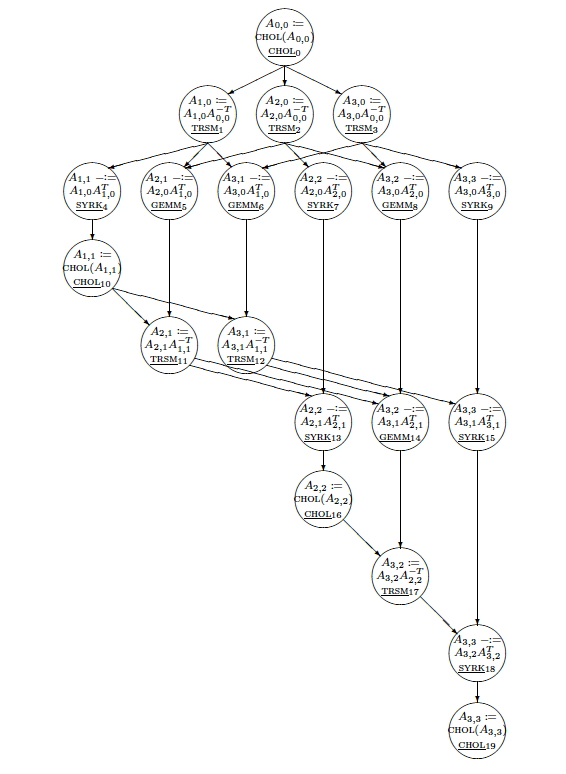
\includegraphics[scale=.25]{chol4dag}
\end{frame}

\begin{frame}{Sometimes\ldots}
  \includegraphics[scale=.06]{mesh3d}
\end{frame}

\begin{frame}{DAG schedulers}
  \begin{itemize}
  \item Directed Acyclic Graph (dataflow)
  \item Each node has dependence on other nodes, can execute when dependencies available
  \item Quark/DaGue (TN): dependence on memory area written \\
    pretty much limited to dense linear algebra
  \item OpenMP has a pretty good scheduler
  \item Distributed memory scheduling is pretty hard
  \end{itemize}
\end{frame}
